\chapter{Design}
Dette kapitel indeholder en beskrivelse af design valgene for Firebase databasen og applikationen, samt hvordan disse er implementeret. \\

\section{Firebase database}

\section{Applikation}
Til udvikling af applikationen er der brugt et MVC design \cite{MVC}, som vist herunder, på figur \ref{fig:MVC}
\begin{figure}[H] % (alternativt [H])
	\centering
	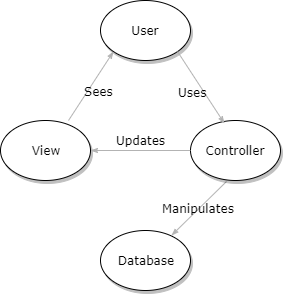
\includegraphics[height=10cm, width=10cm]{../ArkitekturDesign/Design/MVC}
	\caption{MVC design for Rambøll Tilsyn.}
	\label{fig:MVC}
\end{figure}

Model-View-Controller er et design pattern til opbygning af user interfaces. Model er der alt
data ligger. Det er så Controllerens opgave at manipulere det til Viewet. Viewet er det som
ses af brugeren og som der kan interageres med. Hvis brugeren interagerer med applikationen er
det Controllerns opgave at få det ned i Modellen og få kaldt det nye view frem. \\
Der er brugt MVC design pattern til alle views i applikationen.

\clearpage

\section{Login}

\begin{figure}[H] % (alternativt [H])
	\centering
	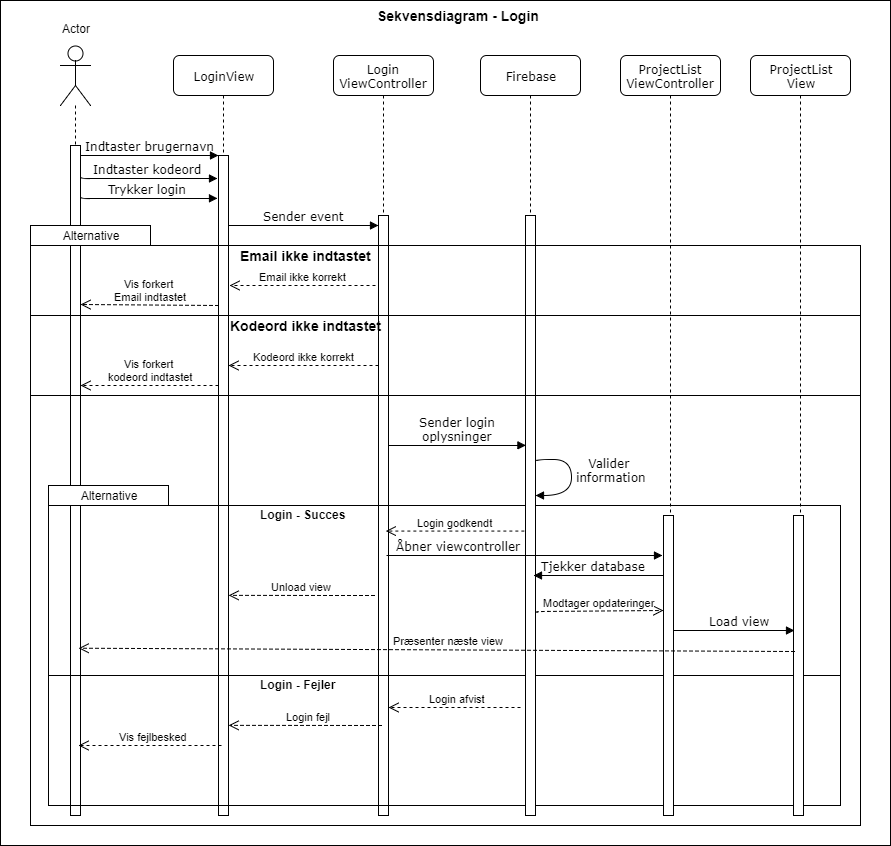
\includegraphics[width=1.1\textwidth]{../ArkitekturDesign/Design/Login/LoginSekvensDiagram}
	\caption{Sekvensdiagram for Login i Rambøll Tilsyn.}
	\label{fig:LoginSekvens}
\end{figure}
\section{Accepttest for Opret bruger (CRS-2)}
Dette afsnit beskriver accepttesten for Opret bruger.

\textbf{User story beskrivelse} \\
Som bruger \\
Ønsker jeg at kunne oprette en bruger på applikationen \\
For at kunne give en anden bruger adgang til systemet

\begin{table}[H]
	\centering
	\begin{tabular}{|ll|l|ll|} \hline
		\textbf{Scenarie} &  & \textbf{Beskrivelse}&  \textbf{Godkendt}&  \\ \hline
		Opret bruger&  &  Når alt information omkring en bruger &  OK&  \\
		& & er udfyldt, og der trykkes opret bruger, bliver brugeren oprettet& & \\ \hline
	\end{tabular}
	\caption{Accepttest for Opret bruger (CRS-2)}
	\label{AcceptOpretBruger}
\end{table}

\clearpage
\section{Accepttest for Opret projekt (CRS-16)}
Dette afsnit beskriver accepttesten for Opret projekt.

\textbf{User story beskrivelse} \\
Som bruger \\
Ønsker jeg at kunne oprette projektoplysninger \\
For at have aktuelle oplysninger om projektet

\begin{table}[H]
	\centering
	\begin{tabular}{|ll|l|ll|} \hline
		\textbf{Scenarie} &  & \textbf{Beskrivelse}&  \textbf{Godkendt}&  \\ \hline
		Opret projekt&  &  Når alt information omkring et projekt &  Ikke OK&  \\
		& & er udfyldt, og der trykkes opret projekt, bliver brugeren oprettet& & \\ \hline
	\end{tabular}
	\caption{Accepttest for Opret projekt (CRS-16)}
	\label{AcceptOpretProjekt}
\end{table}
\subsection{Registrering på PDF}

\subsubsection{Grafisk brugergrænseflade}

\subsubsection{Design \& Implementering}
